\documentclass[11pt,a4paper]{article}

% ---------------------------------------------------------------------------
% Packages
% ---------------------------------------------------------------------------
\usepackage[margin=2.5cm]{geometry}
\usepackage[utf8]{inputenc}
\usepackage[T1]{fontenc}
\usepackage{amsmath,amssymb,amsthm}
\usepackage{booktabs}
\usepackage{caption}
\usepackage{graphicx}
\usepackage{xcolor}
\usepackage{hyperref}
\usepackage[capitalize]{cleveref}
\usepackage{algorithm}
\usepackage{algpseudocode}
\usepackage{tikz}
\usetikzlibrary{positioning,arrows.meta,fit,backgrounds}
\usepackage{pgfplots}
\pgfplotsset{compat=1.18}
\usepackage[font=small,labelfont=bf]{caption}
\usepackage{siunitx}
\sisetup{detect-all,group-separator={,}}

\hypersetup{
  colorlinks=true,
  linkcolor=blue!50!black,
  citecolor=blue!50!black,
  urlcolor=blue!50!black
}

\newtheorem{definition}{Definition}
\newtheorem{remark}{Remark}

\title{\textbf{Cross-Venue Inventory-Aware Market Making for BTC-USD Perpetuals:\\
Design, Iterative Calibration, and Empirical Evaluation of an\\
Avellaneda--Stoikov Quoting System}}

\author{Deniz Gürsu\\
\small Independent Research}

\date{July 2026}

\begin{document}
\maketitle

\begin{abstract}
We present the design, implementation, and empirical evaluation of an automated market-making
system for the BTC-USD perpetual contract on Extended, a StarkEx-based decentralized perpetual
exchange. The strategy quotes around Extended's own order book using an infinite-horizon
Avellaneda--Stoikov (A-S) inventory-risk framework, while using Binance's more liquid BTCUSDT
perpetual market purely as a short-horizon momentum signal rather than as a pricing reference --
a deliberate redesign from an earlier version that anchored quotes to Binance's price and was
found, on live data, to be dominated by a persistent USDT/USD currency basis rather than genuine
edge. We document, in detail, five successive failure modes discovered in the realized-volatility
estimator through live tracing of the venue's WebSocket feed, and the fixes that converged on a
robust, dt-normalized, median-absolute-deviation (MAD) estimator. Because the model's two central
risk parameters -- risk aversion $\gamma$ and order-arrival intensity $\kappa$ -- could not be
reliably estimated from the target venue's own fill data, we replace hand-tuned constants with a
two-level UCB1 contextual-bandit calibration scheme operating over a small, auditable grid, plus
a circuit breaker that forces the model to compete with, or cross, the venue's own book once
inventory has been stuck beyond an empirically observed A-S skew-versus-cross-venue-gap
magnitude mismatch of five to six orders of magnitude. We evaluate the system on
\num{3536771} recorded quote ticks (\num{3397} flush files) gathered over ten days of dry-run
paper trading against real Extended order-book and trade-print data, and present a detailed
case study of a single \num{21.1}-hour continuous session (\num{1246167} ticks,
\num{5883} simulated fills). We report the resulting fill statistics, spread competitiveness
relative to the venue's own touch, and the empirical reward of each explored $(\gamma,\kappa)$
pair, and discuss the strategy's current limitations honestly, including a substantial
intra-session drawdown and the fact that net profitability after fees is not yet consistently
demonstrated.
\end{abstract}

\tableofcontents

% ===========================================================================
\section{Introduction}
% ===========================================================================

Automated market making on centralized and decentralized derivatives venues has become one of
the most heavily studied applications of stochastic optimal control in quantitative finance,
following the seminal inventory-risk formulation of Avellaneda and Stoikov
\cite{avellaneda2008}. The core idea is simple to state: a market maker who posts bid and ask
quotes around a reference (``fair'') price earns the spread on round-trip trades, but accumulates
directional inventory risk whenever order flow is one-sided. The A-S model resolves this by
skewing quotes away from the raw mid-price in proportion to current inventory, risk aversion, and
local volatility, and by widening the spread as a function of the market's own order-arrival
intensity.

This paper documents an end-to-end, from-scratch implementation of that idea for a specific,
concrete, and comparatively under-studied setting: a newly listed, thinly quoted perpetual
market (BTC-USD on Extended, a StarkEx-based perpetual DEX) for which no historical calibration
data exists, alongside a much deeper and more liquid reference market (Binance's BTCUSDT
perpetual future) that trades the same underlying asset but in a different quote currency
(USDT rather than USD) and on a structurally different venue. Unlike textbook treatments of the
A-S model, essentially every input to the model here had to be estimated live, from a feed with
real-world pathologies -- irregular tick spacing, bursty WebSocket delivery, quantity-only book
updates that do not represent genuine price moves, and a persistent cross-venue currency basis --
and every one of those pathologies produced a distinct, diagnosable failure in the resulting
quotes before being fixed. We consider the iterative debugging history itself to be one of the
paper's central contributions: it is a concrete illustration of how far a ``textbook'' market
making formula is from a production-safe implementation, and of the specific empirical checks
that closed that gap.

\subsection{Contributions}
\begin{itemize}
  \item A cross-venue market-making architecture that separates the \emph{pricing reference}
        (the venue actually being quoted on) from a \emph{momentum signal} (a faster, deeper
        market), and a documented empirical finding that collapsing the two -- quoting directly
        on a foreign venue's price -- silently reduces to trading a currency basis rather than
        genuine market-making edge.
  \item A detailed, reproducible account of five iterations of a realized-volatility estimator,
        each triggered by a specific, quantified failure mode observed on live data (\Cref{sec:sigma}).
  \item A two-level adaptive calibration scheme (\Cref{sec:bandit}) that replaces the model's two
        least-observable parameters, $\gamma$ and $\kappa$, with a UCB1 contextual bandit
        \cite{auer2002} over market regime, plus a slower meta-bandit over the bandit's own
        reward-shaping coefficients.
  \item An empirical evaluation on \num{3536771} live-market quote ticks and \num{12983} simulated
        fills, including a full single-session case study with a fee-aware, latency-aware,
        queue-position-aware paper-fill simulator (\Cref{sec:results}), reported with its
        drawdowns and negative periods intact rather than selectively.
\end{itemize}

% ===========================================================================
\section{Related Work}
% ===========================================================================

The theoretical foundation of this work is the inventory-risk market-making model of Avellaneda
and Stoikov \cite{avellaneda2008}, itself building on the earlier dealer-pricing framework of Ho
and Stoll \cite{hostoll1981}. Guéant, Lehalle and Fernández-Tapia \cite{gueant2013} provide a
closed-form approximation to the finite-horizon A-S problem and analyze its asymptotic (infinite
horizon) behavior, which is the regime used in this paper's live implementation, since a
continuously-operating quoting bot has no natural terminal time. Cartea, Jaimungal and Penalva
\cite{cartea2015} and Guéant \cite{gueant2016} give book-length treatments of algorithmic
market-making, order-arrival intensity modeling, and the practical gap between the idealized
Poisson order-flow assumption and observed market microstructure -- a gap this paper reproduces
and quantifies directly on Extended's order flow (\Cref{sec:kappa}). The fair-value construction
used here, the size-weighted \emph{microprice}, follows Stoikov's treatment of the microprice as
a short-horizon predictor of future trade prices \cite{stoikov2018}. The adaptive-parameter
scheme in \Cref{sec:bandit} applies the UCB1 algorithm of Auer, Cesa-Bianchi and Fischer
\cite{auer2002} as a lightweight, auditable alternative to full reinforcement learning for online
hyperparameter selection.

% ===========================================================================
\section{Market Venues, Data, and Microstructure}
\label{sec:data}
% ===========================================================================

\subsection{Trading venues}

The strategy quotes the \texttt{BTC-USD} perpetual contract on \textbf{Extended}, a StarkEx-based
perpetual decentralized exchange, using its public order-book (top-of-book) and public
trade-print WebSocket streams, and (in live mode only) its authenticated account/position stream.
Extended settles and denominates positions in USD. Alongside this, the system subscribes to
Binance's USDT-margined \texttt{BTCUSDT} perpetual \texttt{bookTicker} stream purely as a
secondary signal (\Cref{sec:momentum}) -- \emph{not} as a quoting reference, for reasons detailed
in \Cref{sec:pivot}.

\subsection{The USDT/USD currency basis}
\label{sec:basis}

Binance's BTCUSDT price is denominated in USDT, and USDT does not sit exactly at parity with the
US dollar -- during data collection it traded persistently on the order of several basis points
below real USD. Comparing Binance's raw USDT price against Extended's USD-denominated book
therefore silently mixes currencies. The system corrects for this by polling Binance's own
USDC/USDT spot pair (\texttt{USDCUSDT}, via REST, every \SI{30}{\second}) and treating USDC as a
USD proxy, since USDC trades far closer to parity than USDT does:
\begin{equation}
  \widehat{\text{USD-per-USDT}} = \frac{1}{\tfrac{1}{2}\left(\text{bid}_{\text{USDCUSDT}} +
  \text{ask}_{\text{USDCUSDT}}\right)}.
\end{equation}
Every Binance price used downstream (fair-value comparison and the momentum signal) is converted
through this rate before use. Because this basis moves far more slowly than BTC's own price, a
\SI{30}{\second} polling cadence is sufficient; it is not streamed.

\subsection{Data collection pipeline}

The live quoting process buffers one record per quote-loop tick (nominally every
\SI{50}{\milli\second}; see \Cref{sec:architecture}) containing the fair price, both venues' raw
prices, the momentum signal, the venue's own top-of-book, the model's target quotes, realized
sigma, current inventory and mark-to-market PnL, the currently active $(\gamma,\kappa)$ pair and
market regime, and the currently active bandit reward-shaping coefficients. Buffers are flushed
to an immutable, PID- and epoch-tagged Parquet file every \SI{60}{\second}, written atomically
(temp file plus \texttt{os.replace}) so that a concurrently running read-only dashboard can never
observe a partially written file. This produced the empirical corpus analyzed in
\Cref{sec:results}: \num{3397} flush files totalling \num{3536771} rows, collected across
approximately ten days (2026-07-21 to 2026-07-31) in several dozen discrete sessions as the
model, its parameters, and its bug fixes were iterated.

% ===========================================================================
\section{Strategy Design and Methodology}
\label{sec:methodology}
% ===========================================================================

\subsection{System architecture}
\label{sec:architecture}

The system is a single asyncio event loop running five to six independent coroutines that
communicate through a shared, mutable state object rather than message passing, since all
consumers run in the same process and true concurrency is not required -- only interleaving.
\Cref{fig:architecture} shows the resulting data flow.

\begin{figure}[htbp]
\centering
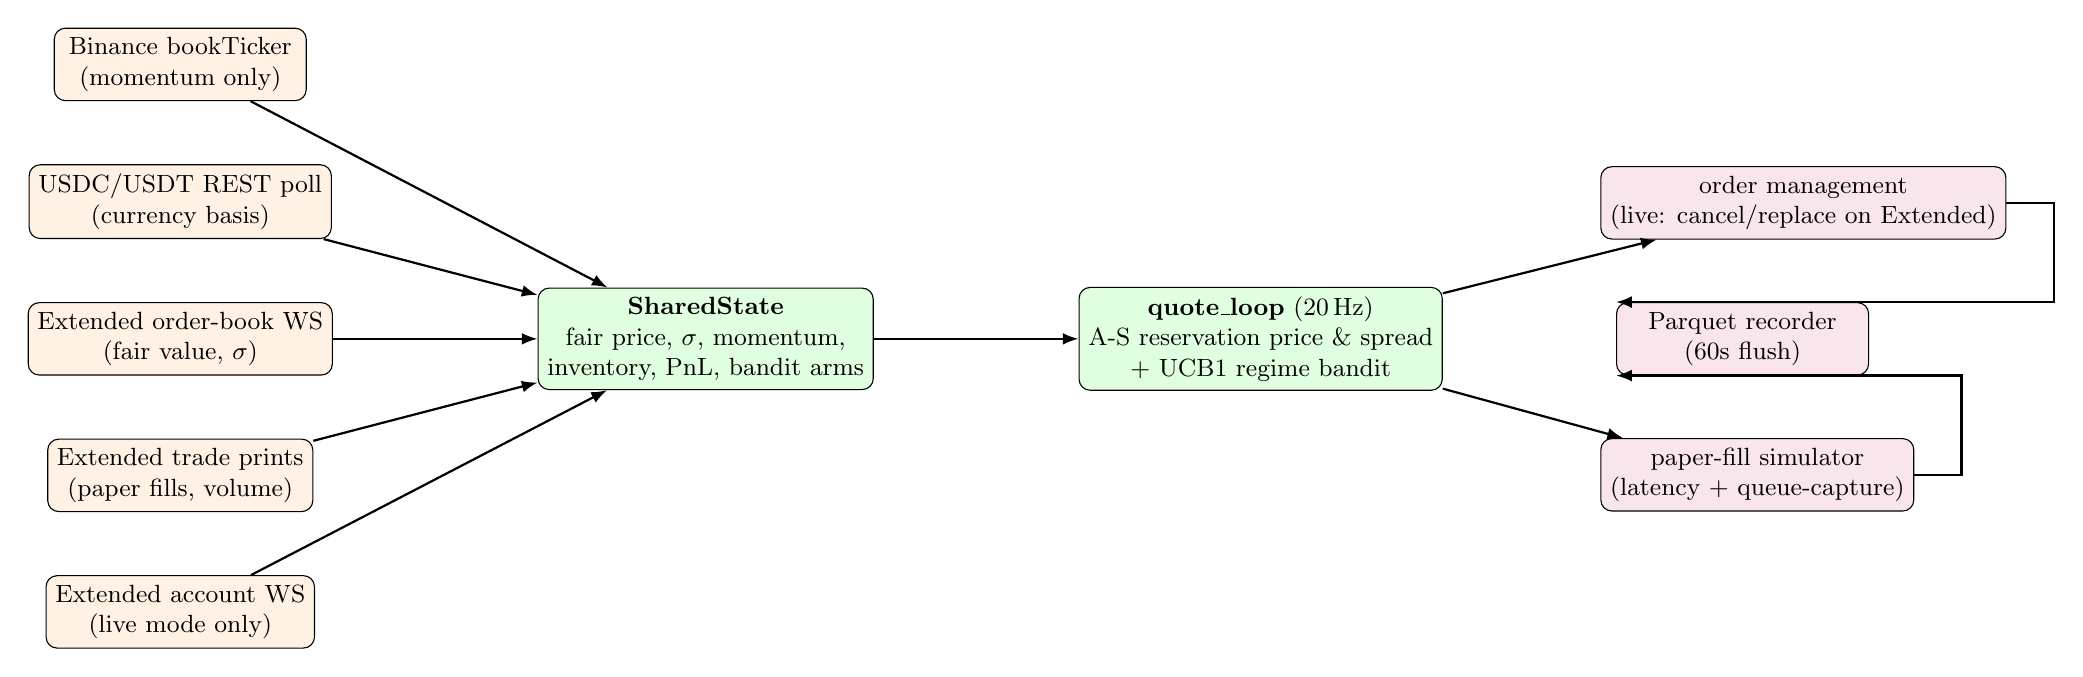
\begin{tikzpicture}[
  node distance=8mm and 12mm,
  box/.style={draw, rounded corners, align=center, minimum height=9mm, minimum width=32mm,
              fill=blue!6, font=\small},
  feed/.style={box, fill=orange!10},
  core/.style={box, fill=green!12, minimum width=38mm},
  sink/.style={box, fill=purple!10},
  arr/.style={-{Latex[length=2mm]}, thick}
]
  \node[feed] (binance) {Binance bookTicker\\(momentum only)};
  \node[feed, below=of binance] (usdt) {USDC/USDT REST poll\\(currency basis)};
  \node[feed, below=of usdt] (extbook) {Extended order-book WS\\(fair value, $\sigma$)};
  \node[feed, below=of extbook] (exttrades) {Extended trade prints\\(paper fills, volume)};
  \node[feed, below=of exttrades] (extacc) {Extended account WS\\(live mode only)};

  \node[core, right=26mm of extbook] (state) {\textbf{SharedState}\\fair price, $\sigma$, momentum,\\inventory, PnL, bandit arms};

  \node[core, right=26mm of state] (loop) {\textbf{quote\_loop} (20\,Hz)\\A-S reservation price \& spread\\+ UCB1 regime bandit};

  \node[sink, above right=6mm and 20mm of loop] (order) {order management\\(live: cancel/replace on Extended)};
  \node[sink, below right=6mm and 20mm of loop] (paper) {paper-fill simulator\\(latency + queue-capture)};

  \node[sink, right=22mm of loop] (rec) {Parquet recorder\\(60s flush)};

  \foreach \f in {binance, usdt, extbook, exttrades, extacc}
    \draw[arr] (\f) -- (state);

  \draw[arr] (state) -- (loop);
  \draw[arr] (loop) -- (order);
  \draw[arr] (loop) -- (paper);
  \draw[arr] (order.east) -- ++(6mm,0) |- (rec.north west);
  \draw[arr] (paper.east) -- ++(6mm,0) |- (rec.south west);
\end{tikzpicture}
\caption{System architecture. Five asynchronous feeds update a shared state object; a single
20\,Hz quote loop reads it, computes Avellaneda--Stoikov quotes under a bandit-selected
$(\gamma,\kappa)$, and either manages real resting orders (\texttt{--live}) or drives a
latency- and queue-position-aware paper-fill simulator (default, dry run). Every tick is
recorded regardless of mode.}
\label{fig:architecture}
\end{figure}

\subsection{From Binance-anchored to Extended-anchored quoting}
\label{sec:pivot}

The system's first design quoted directly around Binance's price on Extended, using Extended's
own market only as the destination for orders. On live data this was found to anchor quotes near
Binance's price even when it persistently differed from Extended's own tradeable book by tens of
dollars, so that orders were routinely either uncompetitive or aggressively marketable relative
to the market they were actually resting on. Once the USDT/USD basis correction in
\Cref{sec:basis} was applied, the residual ``edge'' this produced was found to be smaller than the
round-trip trading fee -- i.e. it was not edge at all, only currency-conversion noise. The system
was redesigned around Extended's own size-weighted microprice as the sole pricing reference:
\begin{equation}
  \mu = \frac{P^{b}Q^{a} + P^{a}Q^{b}}{Q^{a}+Q^{b}},
  \label{eq:microprice}
\end{equation}
where $P^{b},P^{a}$ and $Q^{b},Q^{a}$ are Extended's best bid/ask price and size. This value is
smoothed with an exponential moving average (EMA, $\alpha=0.3$) to obtain the fair price
$s_t$ used by the A-S formula. Binance is retained purely as a faster, deeper leading indicator
(\Cref{sec:momentum}) -- the classical justification for referencing a more liquid market in
market making is adverse-selection defense, not arbitrage, and that is the only role it plays
here.

\subsection{Cross-venue momentum signal}
\label{sec:momentum}

Binance's currency-corrected microprice is smoothed with two EMAs of different speed
($\alpha_{\text{fast}}=0.3$, $\alpha_{\text{slow}}=0.05$); their gap is a simple momentum / lead
estimate,
\begin{equation}
  m_t = \text{EMA}_{\text{fast}}(t) - \text{EMA}_{\text{slow}}(t),
\end{equation}
which is zero if Binance data is stale (older than \SI{1}{\second}) or unavailable. $m_t$ enters
the reservation price directly, in dollars (\Cref{eq:reservation}), deliberately \emph{not}
routed through the $\gamma\sigma^{2}$ inventory-skew channel: an early diagnostic
(\Cref{sec:limitations}) found that channel to be roughly five to six orders of magnitude too
weak, at the calibrated parameter values, to move the reservation price meaningfully -- a direct
dollar pass-through was the only way to make the signal have any effect on quotes at all.

\subsection{Volatility estimation: five iterations to a robust estimator}
\label{sec:sigma}

Estimating $\sigma$ -- the realized dollar volatility of Extended's own price -- from a live,
irregularly-sampled WebSocket feed turned out to be the single most failure-prone component of
the system. \Cref{tab:sigma-iterations} summarizes the five distinct failure modes discovered, in
order, each found through direct tracing of a live run rather than by inspection of the formula
alone.

\begin{table}[htbp]
\centering
\small
\caption{Iterative development of the realized-volatility estimator. Each row is a distinct
failure mode discovered on live data, in chronological order.}
\label{tab:sigma-iterations}
\begin{tabular}{@{}p{0.10\linewidth}p{0.32\linewidth}p{0.28\linewidth}p{0.24\linewidth}@{}}
\toprule
\textbf{Iter.} & \textbf{Symptom} & \textbf{Root cause} & \textbf{Fix} \\
\midrule
1 & \texttt{target\_ask} briefly hit \$79{,}773 vs.\ a true price of $\approx$\$66{,}600 &
  One sample with an outsized \emph{dt} (e.g.\ a multi-second reconnect gap) pooled against many
  tiny-\emph{dt} samples in a plain $\mathrm{std}(\text{diffs})/\sqrt{\overline{dt}}$ estimator,
  inflating $\sigma$ by $\sim\!600\times$ for the following $\sim\!200$ ticks &
  Normalize \emph{each} sample by its own \emph{dt} before taking a dispersion statistic \\
\addlinespace
2 & $\sigma$ pinned at $149$ on a provably static book; quotes widened to \$2{,}000+ from fair &
  Extended's WebSocket sometimes delivers bursts with microsecond-scale gaps
  ($\sim\!2\times10^{-5}\,\text{s}$, not the assumed $\sim\!50\,\text{ms}$); a real few-cent diff
  divided by $\sqrt{dt\to 0}$ explodes &
  Floor \emph{dt} at $\mathtt{MIN\_TICK\_DT\_SEC}=\SI{5}{\milli\second}$ before normalizing \\
\addlinespace
3 & $\sigma$ spiked to $\sim\!30$ against a $\sim\!2$ baseline mid-unwind, from a 40-min run &
  Even with the \emph{dt} floor, a couple of genuinely fast \$0.50--\$1 real moves get amplified
  by $1/\sqrt{dt}$ into normalized values $10$--$15\times$ typical, and plain $\mathrm{std}(\cdot)$
  lets a handful of outliers dominate a 200-sample window &
  Replace $\mathrm{std}(\cdot)$ with a normality-scaled median absolute deviation (MAD),
  $\hat\sigma = 1.4826\cdot\mathrm{median}(|x_i-\mathrm{median}(x)|)$ \\
\addlinespace
4 & $\sigma$ collapsed back to $\sim\!0.087$ (pre-fix level) despite the MAD fix &
  $>\!50\%$ of consecutive book ticks are quantity-only updates with an exact-zero microprice
  diff; once a majority of a 200-sample window is a repeated value, the median -- and MAD, built
  from it -- collapses toward it &
  Filter exact-zero diffs at compute time \\
\addlinespace
5 & Same collapse persisted ($\sigma_{\$}$ pinned $\approx\!0.08$ vs.\ $\approx\!2.1$ before);
  target spread flatlined regardless of real volatility &
  $67\%$ of ticks still showed sub-\$0.001 microprice ``moves'' from qty-only changes at an
  \emph{unchanged} price level -- the qty-weighted microprice wobbles even when the touch itself
  does not move &
  Feed $\sigma$ off the plain \emph{price-level} mid $(P^b{+}P^a)/2$, which only updates when the
  touch genuinely moves (confirmed: $1.4\%$ of raw ticks); the qty-weighted microprice is kept
  \emph{only} for the fair-value/quoting reference, where its wobble is legitimate signal \\
\bottomrule
\end{tabular}
\end{table}

The final estimator (\Cref{alg:sigma}) maintains a rolling window of the last \texttt{VOL\_WINDOW}$=200$
genuine price-level moves (not messages), each paired with the wall-clock time since the
\emph{previous} genuine move, floored at \texttt{MIN\_TICK\_DT\_SEC}. It requires at least 20
samples before returning a value, so the strategy simply does not quote until enough real
price-level history has accumulated.

\begin{algorithm}[htbp]
\caption{Realized dollar volatility estimator (final version)}
\label{alg:sigma}
\begin{algorithmic}[1]
\Function{OnBookUpdate}{$P^b, Q^b, P^a, Q^a$}
  \State $\mu \gets$ microprice via \Cref{eq:microprice} \Comment{used for fair value, not $\sigma$}
  \State $\text{fair} \gets \text{EMA}_{\alpha=0.3}(\mu)$
  \State $m \gets (P^b+P^a)/2$ \Comment{price-level mid: only moves on genuine touch changes}
  \If{$m \neq \text{last\_mid}$}
     \State $dt \gets \text{now} - \text{last\_mid\_ts}$
     \If{$dt > 0$}
        \State append $(m - \text{last\_mid})$ to \textsc{PriceDiffs}; append $dt$ to \textsc{TickDts}
     \EndIf
     \State $\text{last\_mid} \gets m$;\ \ $\text{last\_mid\_ts} \gets \text{now}$
  \EndIf
\EndFunction
\Statex
\Function{RealizedSigmaDollar}{}
  \If{$|\textsc{PriceDiffs}| < 20$} \Return \textsc{None} \EndIf
  \State $dt_i \gets \max(\textsc{TickDts}_i,\ \texttt{MIN\_TICK\_DT\_SEC})\ \ \forall i$
  \State $x_i \gets \textsc{PriceDiffs}_i / \sqrt{dt_i}$
  \State $\hat\sigma \gets 1.4826 \cdot \mathrm{median}(|x_i - \mathrm{median}(x)|)$
  \State \Return $\hat\sigma$
\EndFunction
\end{algorithmic}
\end{algorithm}

\subsection{Order-arrival intensity $\kappa$}
\label{sec:kappa}

In the A-S model, $\kappa$ parametrizes an assumed exponential decay of fill probability with
distance from the mid-price. It was first calibrated offline, in an exploratory notebook, as
$\kappa = 1/\overline{|P_{\text{trade}} - \text{mid}|}$ over Binance's own trade flow -- a deep
market with an average trade-to-mid distance of $\approx\!\$5.50$. Deployed as-is against
Extended, this implied a spread nowhere near competitive with Extended's own $\approx\!\$1$
market, and was confirmed live to produce a stable but roughly $9\times$-too-wide $\approx\!\$9$
spread that was never filled. A regression fit against Extended's own realized fills later gave
$\hat\kappa\approx 0.51$, but the underlying empirical fill-probability-vs-distance shape was
found to look like a step (a ``cliff'' at the touch) rather than the smooth exponential decay the
model assumes, so this fitted value was judged untrustworthy and not used directly. In its place,
$\kappa$ is treated as a free parameter selected online by the bandit in \Cref{sec:bandit}, seeded
at a value ($\kappa_0=5.0\,\text{USD}^{-1}$) chosen to imply an average fillable distance
comparable to Extended's own spread, and swept over a small explicit candidate grid rather than
estimated from a mis-specified parametric model.

\subsection{Quoting formula}
\label{sec:quotes}

The live system uses the stationary (infinite-horizon) approximation to the A-S problem -- there
is no $(T-t)$ decay term, since the strategy quotes continuously with no natural session end. Note
this differs from the finite-horizon formulation originally used to validate $\gamma$ offline
(\Cref{sec:calibration-history}); the sigma/kappa units are shared, but the horizon treatment is
not. Given fair price $s_t$, signed inventory $q_t$, and momentum skew $m_t$:
\begin{align}
  r_t &= s_t - q_t\,\gamma\,\sigma_t^{2} + m_t, \label{eq:reservation}\\
  \delta_t &= \gamma\,\sigma_t^{2} + \frac{2}{\gamma}\ln\!\left(1+\frac{\gamma}{\kappa}\right),
    \label{eq:spread}\\
  \text{bid}_t &= r_t - \delta_t/2, \qquad \text{ask}_t = r_t + \delta_t/2. \label{eq:quotes}
\end{align}
$r_t$ is the reservation (indifference) price and $\delta_t$ the total optimal spread. Every
quote tick is checked against a hard sanity bound
($|\text{bid}_t - s_t|/s_t \le \texttt{MAX\_QUOTE\_DEVIATION\_PCT}=2\%$, and symmetrically for the
ask) before use, discarding the tick otherwise; this bound was added directly in response to
Iteration~1 in \Cref{tab:sigma-iterations}, as a second, independent line of defense against any
future volatility-estimator regression.

\subsection{Risk management}
\label{sec:risk}

Three mechanisms bound the strategy's risk independently of the A-S formula itself:

\paragraph{Inventory cap.} No new quote is added on a side once $|q_t|$ would exceed
\texttt{MAX\_INVENTORY}; the corresponding side is instead withdrawn.

\paragraph{Requote throttling.} Orders are only cancelled/replaced if the new target price moves
by more than \texttt{REPRICE\_THRESHOLD\_BPS} (2\,bps) from the currently resting price, and no
more often than every \texttt{MIN\_REQUOTE\_INTERVAL\_SEC} (\SI{0.5}{\second}), independent of the
20\,Hz quote-computation cadence, to bound order-book churn.

\paragraph{Stuck-inventory circuit breaker.} A live diagnostic found that the A-S inventory-skew
term moves the reservation price by only $q\,\gamma\,\sigma^{2}\approx\$0.0001$ at the maximum
allowed position, against typical Binance-vs-Extended structural gaps of tens of dollars -- a
mismatch of five to six orders of magnitude, meaning the vanilla model can never, on its own,
bridge a genuinely structural (non-noise) price gap, and a position can in principle sit stuck
indefinitely. \Cref{alg:unwind} formalizes the resulting three-stage override: once inventory has
failed to shrink for \texttt{STUCK\_WARN\_SEC} (\SI{300}{\second}), the exit side is repriced to
join Extended's own top-of-book (still passive); after \texttt{STUCK\_FORCE\_SEC}
(\SI{1200}{\second}) it is submitted without \texttt{post\_only}, deliberately crossing the
spread to guarantee an exit. A related, non-obvious defect surfaced during development: the
override reprices only the exit side, independently of the (still-normal) other side, and a real
run showed the two can cross -- e.g.\ momentum pushing the normal bid up at the same tick the
override pulled the ask down to Extended's ask, producing bid~$\ge$~ask. An un-crossing check was
added so a crossed pair can never reach either the paper-fill simulator or a real order.

\begin{algorithm}[htbp]
\caption{Stuck-inventory circuit breaker}
\label{alg:unwind}
\begin{algorithmic}[1]
\State $t_{\text{stuck}} \gets \text{now} - \text{last\_unwind\_ts}$ \Comment{reset whenever $|q_t|$ shrinks or hits 0}
\If{$q_t = 0$} \State stage $\gets$ \textsc{None}
\ElsIf{$t_{\text{stuck}} \ge \texttt{STUCK\_FORCE\_SEC}$} \State stage $\gets$ \textsc{Force}
\ElsIf{$t_{\text{stuck}} \ge \texttt{STUCK\_WARN\_SEC}$} \State stage $\gets$ \textsc{Warn}
\Else \State stage $\gets$ \textsc{None}
\EndIf
\If{stage $\ne$ \textsc{None} and Extended's book is known}
  \If{$q_t > 0$} \Comment{long: exit side is the ask}
     \State ask $\gets$ (stage $=$ \textsc{Force}) ? Extended's own bid, submitted taker
                        : Extended's own ask, submitted maker
  \Else \Comment{short: exit side is the bid}
     \State bid $\gets$ (stage $=$ \textsc{Force}) ? Extended's own ask, submitted taker
                        : Extended's own bid, submitted maker
  \EndIf
\EndIf
\If{bid $\ge$ ask} \State \textbf{skip this tick entirely} \Comment{never emit a crossed pair}
\EndIf
\end{algorithmic}
\end{algorithm}

\subsection{Adaptive calibration: a two-level UCB1 bandit}
\label{sec:bandit}

Because neither $\gamma$ nor $\kappa$ could be reliably estimated from Extended's own fill data
(\Cref{sec:kappa}), and because their hand-tuned history (\Cref{sec:calibration-history}) required
manual re-tuning every time market conditions changed, both are instead selected online by a
UCB1 contextual bandit \cite{auer2002} over a small candidate grid,
$\gamma\in\{0.002,0.005,0.01\}$, $\kappa\in\{1.0,5.0,20.0\}$ (each trimmed down from a wider grid
once early runs showed $\gamma=0.02$ dominated by every other value it was paired with, so as to
let the bandit finish exploring, and start exploiting, within a realistic session length). One
independent arm-statistics table is kept per \emph{market regime} -- the trailing-percentile
33/67 buckets (low/mid/high) of realized $\sigma$ crossed with trailing-percentile buckets of
recent traded volume, so the definition of ``normal'' adapts as the market's own range drifts over
a long deployment, rather than encoding a fixed assumption:
\begin{equation}
  \text{regime}_t = \text{bucket}_{33/67}(\sigma_t)\ \times\ \text{bucket}_{33/67}(\text{vol}_t),
\end{equation}
where $\text{vol}_t$ is trade quantity summed over the trailing \SI{60}{\second}. An arm's UCB1
score in regime $\rho$ is
\begin{equation}
  \text{UCB}(\gamma,\kappa\mid\rho) = \hat\mu_{\rho,\gamma,\kappa} +
    c\sqrt{\frac{\ln N_\rho}{n_{\rho,\gamma,\kappa}}},
\end{equation}
with exploration constant $c=2.0$; an arm never tried in the current regime is always selected
first, so a brand-new regime sweeps the full $3\times3$ grid before exploiting. The chosen arm is
held for \texttt{BANDIT\_EVAL\_WINDOW\_SEC} (\SI{120}{\second}) and then scored by
\begin{equation}
  \text{reward} = \Delta\text{PnL} + \beta_{\text{fill}}\cdot(\text{fills in window})
    - \beta_{\text{inv}}\cdot|q_{\text{window-end}}|\cdot\sigma,
  \label{eq:reward}
\end{equation}
i.e.\ realized PnL change over the window, plus a bonus per fill (to keep generating fill data
while the PnL signal is still thin, early in a deployment), minus a penalty on inventory left open
\emph{at window close} (not its peak, since PnL is already mark-to-market and would already
reflect a position that spiked and was unwound \emph{within} the window), scaled by $\sigma$ since
a given leftover position is riskier in a more volatile regime. The reward-shaping coefficients
$(\beta_{\text{fill}}, \beta_{\text{inv}})$ are themselves picked by a second, slower, global (not
regime-conditioned) UCB1 bandit over the candidate sets $\beta_{\text{fill}}\in\{0,0.05,0.15\}$,
$\beta_{\text{inv}}\in\{0,0.5,1.0,2.0\}$, re-scored every \texttt{COEF\_EVAL\_WINDOW\_SEC}
(\SI{1800}{\second}) using \emph{raw} PnL delta rather than the shaped reward those coefficients
themselves define -- judging a coefficient choice by a metric it controls would be circular. Both
bandits persist their learned statistics to disk as plain JSON, deliberately, so that a
restart resumes rather than re-exploring from scratch, and so the state can be inspected or reset
by hand.

We chose a small, auditable two-level UCB1 scheme over a full reinforcement-learning policy
deliberately: with only two parameters, a slowly shifting regime, and a strong preference for
being able to explain \emph{why} a given quote was chosen, a bandit whose entire state is a
human-readable table of (regime, arm) $\to$ (count, mean reward) was judged preferable to an
opaque trained policy, even at the cost of asymptotic optimality.

\subsection{Calibration history}
\label{sec:calibration-history}

\Cref{tab:calibration-history} traces the evolution of $\gamma$ and $\kappa$ from their first
offline calibration through to the adaptive scheme of \Cref{sec:bandit}, illustrating how far a
single offline-fitted value was from being usable once deployed against a different, thinner
market.

\begin{table}[htbp]
\centering
\small
\caption{Calibration history of $\gamma$ and $\kappa$.}
\label{tab:calibration-history}
\begin{tabular}{@{}p{0.16\linewidth}p{0.14\linewidth}p{0.14\linewidth}p{0.5\linewidth}@{}}
\toprule
\textbf{Stage} & $\gamma$ & $\kappa$ (USD) & \textbf{Note} \\
\midrule
Offline (finite horizon, Binance-anchored) & $0.09$ & $0.18$ & Swept offline in a notebook
  against a different (finite-horizon, Binance-mid) formulation than the one later deployed. \\
First live deployment & $0.09$ & $0.18$ & Once the volatility estimator was fixed (mean
  $\sigma\approx 6.57$, vs. the broken estimator's $\approx 0.08$), $\gamma\sigma^2$ alone
  reached $\approx\$3.88$ -- already exceeding the entire distance range at which fills occur at
  all on Extended (fill rate $\approx 15$--$25\%$ inside the touch, indistinguishable from zero
  past $\$0.50$). \\
Manual correction & $0.02$ & $0.18$ & Places the inventory floor ($\approx\$0.86$ at that
  $\sigma$) inside the empirically fillable range; a reasoned starting point, not a fitted one. \\
Backtesting/data-gathering & $0.005$ & $5.0$ & Deliberately loosened for more fill volume,
  putting the modeled spread at $\approx\$0.5$--$1.2$ across the observed $\sigma$ range
  ($3.8$--$12.5$), at or tighter than Extended's own $\approx\$1$ touch. \\
Adaptive (current) & bandit-selected $\in\{0.002,0.005,0.01\}$ &
  bandit-selected $\in\{1.0,5.0,20.0\}$ & See \Cref{sec:bandit}; the values above become only the
  bandit's seed before its first evaluation window closes. \\
\bottomrule
\end{tabular}
\end{table}

\subsection{Execution and fee simulation (dry run)}
\label{sec:execution-sim}

In the default, credential-free dry-run mode, the system does not place real orders; instead it
paper-fills against Extended's own real trade prints. Three effects that a naive
``instantly and fully fillable'' simulation would miss are modeled explicitly:

\begin{itemize}
  \item \textbf{Network/cancel latency.} A decided quote is not treated as resting until
        \texttt{NETWORK\_LATENCY\_SEC} ($\SI{8.5}{\milli\second}$) after it is computed, and a
        superseded quote remains fillable for \texttt{CANCEL\_LATENCY\_SEC}
        ($\SI{4}{\milli\second}$) after being replaced, mirroring the fact that a real order has
        to travel to the exchange before it is live or gone.
  \item \textbf{Queue position / capture ratio.} Not every real trade that crosses our resting
        price would, in reality, reach our specific order, since other resting orders at the
        same price level and faster participants are served first. Lacking Extended's private L3
        queue-position feed, this is treated as a swept sensitivity parameter,
        \texttt{TRADE\_CAPTURE\_RATIO}$\in\{0.2,0.5,0.7,1.0\}$: only that fraction of a
        qualifying public trade's quantity is assumed to reach our order.
  \item \textbf{Fees.} A negotiated maker rate of $-1.3$\,bps (a rebate, credited on every
        passive fill) and a taker rate of $2.25$\,bps (charged only on the circuit breaker's
        forced-cross exits) are applied per fill, matching Extended's confirmed live rate.
\end{itemize}

Each simulated resting order (\texttt{PaperRestingOrder}) tracks remaining fillable size
independently for its current price and, during a cancel/replace handoff, its just-superseded
price, so a single trade print can consume at most one order's worth of size, the same way a real
resting order would be exhausted rather than infinitely refillable.

% ===========================================================================
\section{Backtesting and Empirical Results}
\label{sec:results}
% ===========================================================================

All results in this section are computed on real Extended and Binance market data captured live;
no synthetic or resampled data is used. We report both (i) descriptive statistics pooled across
the full ten-day corpus, and (ii) a detailed case study of a single, uninterrupted 21.1-hour
session, since pooling many short, differently-parametrized sessions into one time series can
otherwise obscure -- or, in the case of fill counts, actively corrupt, since several sessions ran
as concurrent sweep processes over the same wall-clock interval -- what any single deployment
actually experienced.

\subsection{Dataset}

\Cref{tab:dataset} summarizes the full corpus and the case-study session used for the equity-curve
analysis below.

\begin{table}[htbp]
\centering
\small
\caption{Empirical dataset summary.}
\label{tab:dataset}
\begin{tabular}{@{}lrr@{}}
\toprule
& \textbf{Full corpus} & \textbf{Case-study session} \\
\midrule
Period & 2026-07-21 -- 2026-07-31 & 2026-07-30, 21.1\,h continuous \\
Flush files / process & \num{3397} files & single PID, uninterrupted \\
Quote-loop ticks & \num{3536771} & \num{1246167} \\
Mode & dry run (paper fills) & dry run (paper fills) \\
Trade-capture ratio & $\{0.2,0.5,0.7,1.0\}$ (swept) & $1.0$ \\
Simulated fills (buy/sell) & \num{6861} / \num{6122} (\num{12983} total) & \num{3185} / \num{2698}
  (\num{5883} total) \\
Fill rate (ticks with a fill) & $0.37\%$ & $0.47\%$ \\
\bottomrule
\end{tabular}
\end{table}

\begin{remark}
An earlier pass over this data computed fill counts by differencing the \texttt{inventory} column
of the full, wall-clock-sorted table directly, without first grouping by writer process. Because
several sessions in the corpus were deliberately run \emph{concurrently} (to sweep
\texttt{--capture-ratio} against the same live market), that naive diff interleaves independent
processes' inventory series and reports spurious ``fills'' at every process handoff, overstating
the true fill count by roughly $35\times$ (\num{460800} vs.\ the correct \num{12983}). All figures
reported in this section are computed after grouping by writer PID first. We flag this explicitly
because it is exactly the kind of silent aggregation error the rest of this paper argues live
systems are prone to, and it is worth naming even in the paper's own analysis code.
\end{remark}

\subsection{Volatility and spread}

Over the case-study session, realized $\sigma_{\$}$ (\Cref{alg:sigma}) had mean \$6.84 and median
\$6.86 (full-corpus mean \$6.80), consistent across the two samples despite the corpus spanning
many different market conditions and bandit generations. Our own quoted spread had mean \$0.74
and median \$0.69, against Extended's own top-of-book spread, mean \$1.01 and median \$1.00 --
i.e.\ over this session the strategy quoted, on average, about $27\%$ \emph{tighter} than
Extended's own resting book. \Cref{fig:sigma} shows the realized-$\sigma$ trajectory over the
session.

\begin{figure}[htbp]
\centering
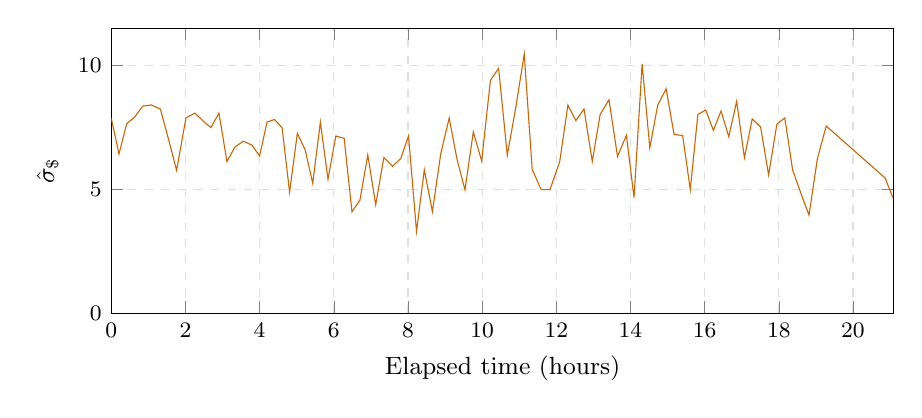
\begin{tikzpicture}
\begin{axis}[
  width=0.95\linewidth, height=5.2cm,
  xlabel={Elapsed time (hours)}, ylabel={$\hat\sigma_{\$}$},
  grid=major, grid style={dashed,gray!25},
  xmin=0, xmax=21.1, ymin=0,
  tick label style={font=\footnotesize}, label style={font=\small}
]
\addplot[thin, color=orange!80!black] coordinates {
(0.0,7.86) (0.208,6.42) (0.415,7.641) (0.626,7.903) (0.849,8.351) (1.076,8.4) (1.324,8.234)
(1.538,7.047) (1.761,5.76) (2.013,7.877) (2.253,8.07) (2.474,7.756) (2.686,7.485) (2.903,8.071)
(3.119,6.114) (3.338,6.708) (3.561,6.935) (3.789,6.781) (3.999,6.344) (4.2,7.708) (4.403,7.811)
(4.606,7.476) (4.808,4.881) (5.017,7.256) (5.226,6.595) (5.432,5.237) (5.638,7.708) (5.843,5.401)
(6.055,7.146) (6.279,7.053) (6.49,4.092) (6.704,4.553) (6.916,6.384) (7.13,4.374) (7.35,6.281)
(7.584,5.925) (7.805,6.236) (8.015,7.148) (8.231,3.3) (8.441,5.78) (8.659,4.099) (8.884,6.436)
(9.112,7.868) (9.325,6.192) (9.537,4.976) (9.762,7.312) (9.988,6.138) (10.223,9.386) (10.445,9.878)
(10.678,6.37) (10.904,8.266) (11.135,10.449) (11.35,5.797) (11.591,4.985) (11.83,4.985)
(12.092,6.114) (12.312,8.389) (12.527,7.767) (12.747,8.235) (12.97,6.124) (13.183,8.015)
(13.421,8.606) (13.65,6.322) (13.89,7.173) (14.096,4.663) (14.314,10.053) (14.521,6.67)
(14.734,8.387) (14.962,9.049) (15.175,7.213) (15.407,7.162) (15.613,4.983) (15.817,8.015)
(16.03,8.195) (16.235,7.373) (16.442,8.154) (16.65,7.118) (16.863,8.543) (17.073,6.27)
(17.283,7.839) (17.51,7.504) (17.725,5.576) (17.947,7.62) (18.162,7.877) (18.372,5.778)
(18.594,4.842) (18.814,3.953) (19.041,6.237) (19.278,7.549) (20.867,5.452) (21.074,4.66)
};
\end{axis}
\end{tikzpicture}
\caption{Realized dollar volatility $\hat\sigma_{\$}$ (MAD-based estimator, \Cref{alg:sigma}) over
the 21.1-hour case-study session. The estimator stays within a stable $\approx\$4$--$10$ band
with no pathological spikes, in contrast to the failure modes of \Cref{tab:sigma-iterations}.}
\label{fig:sigma}
\end{figure}

\subsection{Case-study equity curve}
\label{sec:equity-curve}

\Cref{fig:pnl} shows fee-aware, mark-to-market paper PnL over the case-study session. The
strategy accumulates steadily from \$0 to a peak of \$\num{195.74} around hour 15.8, then
experiences a sharp drawdown to a session low of $-\$\num{112.40}$ (a $\approx\$308$ peak-to-trough
move) by hour 17.1, before partially recovering and closing the session at $-\$6.70$.

\begin{figure}[htbp]
\centering
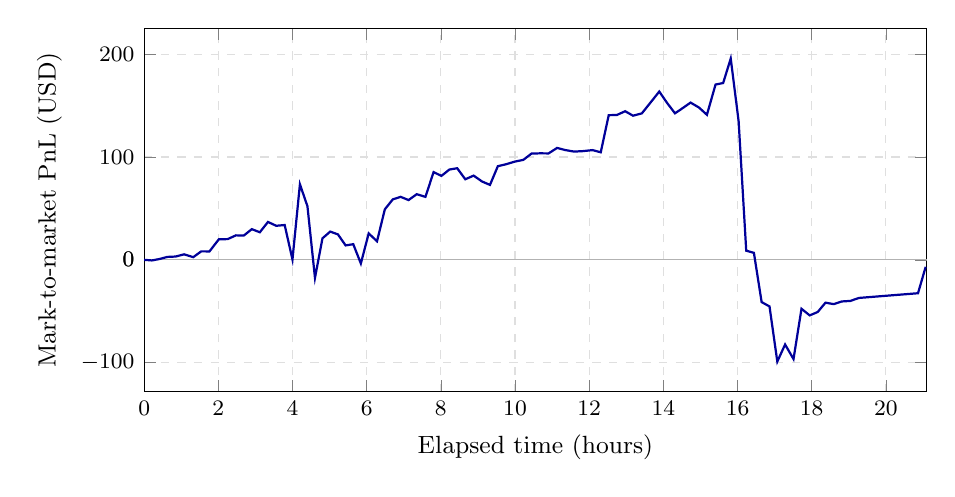
\begin{tikzpicture}
\begin{axis}[
  width=0.95\linewidth, height=6.2cm,
  xlabel={Elapsed time (hours)}, ylabel={Mark-to-market PnL (USD)},
  grid=major, grid style={dashed,gray!25},
  xmin=0, xmax=21.1,
  tick label style={font=\footnotesize}, label style={font=\small},
  extra y ticks={0}, extra y tick style={grid=major,grid style={solid,gray!60}}
]
\addplot[thick, color=blue!60!black] coordinates {
(0.0,0.0) (0.208,-0.58) (0.415,0.82) (0.626,2.85) (0.849,3.21) (1.076,5.36) (1.324,2.61)
(1.538,8.23) (1.761,8.2) (2.013,19.94) (2.253,20.17) (2.474,23.81) (2.686,23.6) (2.903,29.83)
(3.119,26.81) (3.338,36.83) (3.561,33.11) (3.789,33.87) (3.999,0.29) (4.2,73.5) (4.403,52.1)
(4.606,-17.53) (4.808,20.92) (5.017,27.47) (5.226,24.73) (5.432,14.01) (5.638,15.23) (5.843,-3.54)
(6.055,25.7) (6.279,18.07) (6.49,49.13) (6.704,58.79) (6.916,61.25) (7.13,58.13) (7.35,63.83)
(7.584,61.24) (7.805,85.32) (8.015,81.61) (8.231,87.81) (8.441,89.09) (8.659,78.35) (8.884,81.89)
(9.112,76.17) (9.325,72.86) (9.537,91.04) (9.762,92.98) (9.988,95.46) (10.223,97.19)
(10.445,103.31) (10.678,103.57) (10.904,103.48) (11.135,108.82) (11.35,106.79) (11.591,105.25)
(11.83,105.71) (12.092,106.7) (12.312,104.57) (12.527,140.66) (12.747,140.85) (12.97,144.51)
(13.183,140.15) (13.421,142.43) (13.65,152.75) (13.89,163.65) (14.096,152.81) (14.314,142.47)
(14.521,147.52) (14.734,152.91) (14.962,148.06) (15.175,141.03) (15.407,170.43) (15.613,171.95)
(15.817,195.74) (16.03,134.75) (16.235,8.9) (16.442,6.79) (16.65,-41.06) (16.863,-45.33)
(17.073,-98.92) (17.283,-82.33) (17.51,-96.46) (17.725,-47.61) (17.947,-54.03) (18.162,-50.71)
(18.372,-41.66) (18.594,-43.04) (18.814,-40.46) (19.041,-39.95) (19.278,-37.03) (20.867,-32.46)
(21.074,-6.78)
};
\end{axis}
\end{tikzpicture}
\caption{Fee-aware, mark-to-market paper PnL over the 21.1-hour case-study session
(\num{1246167} ticks, \num{5883} simulated fills, trade-capture ratio $1.0$). PnL accumulates
steadily for the first $\approx 16$ hours, then gives back roughly $60\%$ of its peak in a single
$\approx$1.3-hour drawdown before partially recovering.}
\label{fig:pnl}
\end{figure}

We report this drawdown in full rather than truncating the session at its peak. The bandit's
regime bucketing (\Cref{sec:bandit}) is defined against \emph{trailing} percentiles of $\sigma$
and volume, so a genuine, sustained regime shift -- rather than a single bad tick, which the
sanity bound in \Cref{sec:quotes} would already reject -- can still momentarily leave the
currently-held $(\gamma,\kappa)$ arm poorly suited to the new regime until the next
\SI{120}{\second} evaluation window closes and a new arm is selected; \Cref{fig:sigma} shows no
corresponding spike in $\hat\sigma_{\$}$ at hour $\approx 16$--17, suggesting the drawdown is more
consistent with a directional order-flow imbalance (a run of same-side fills) than with a
volatility regime change the model failed to detect.

\subsection{Fill and quoting activity}

Across the case-study session, \num{5883} simulated fills occurred (\num{3185} buy, \num{2698}
sell) -- close to balanced, consistent with the inventory-skew term in \Cref{eq:reservation}
doing its intended directional job rather than the strategy accumulating a persistent one-sided
position. The circuit breaker of \Cref{alg:unwind} activated its \textsc{Warn} stage on $2.6\%$
of ticks and its \textsc{Force} stage (a deliberate, fee-paying cross) on only $0.15\%$ of ticks,
indicating that under normal conditions the vanilla A-S inventory skew, together with ordinary
two-sided fill flow, was sufficient to keep inventory moving without needing to force an exit.

\subsection{Sensitivity to queue-position assumptions}

\Cref{tab:capture-ratio} reports mean paper PnL per tick across the four swept values of the
trade-capture ratio (\Cref{sec:execution-sim}). Average PnL increases with the assumed capture
fraction across this sample, i.e.\ under the negotiated fee structure (a $-1.3$\,bps maker
rebate), capturing a larger share of each qualifying crossing trade was, on average, favorable
rather than adversely selected in this dataset. We note the $0.2/0.5/0.7$ sweeps are much shorter
sessions ($\approx\SI{124}{k}$ ticks each) than the $1.0$ regime ($\approx\SI{2.05}{M}$ ticks,
which also contains the case-study session and most of the corpus's post-drawdown history), so
this is a suggestive rather than a tightly controlled comparison.

\begin{table}[htbp]
\centering
\small
\caption{Mean paper PnL by trade-capture ratio (full corpus, pooled across all sessions at that
ratio).}
\label{tab:capture-ratio}
\begin{tabular}{@{}rrr@{}}
\toprule
\textbf{Capture ratio} & \textbf{Ticks} & \textbf{Mean PnL (USD)} \\
\midrule
$0.2$ & \num{123586} & \num{2.34} \\
$0.5$ & \num{124484} & \num{6.37} \\
$0.7$ & \num{124654} & \num{7.51} \\
$1.0$ & \num{2052985} & \num{30.38} \\
\bottomrule
\end{tabular}
\end{table}

\subsection{Bandit arm performance by $(\gamma,\kappa)$}

\Cref{tab:bandit-arms} aggregates the persisted bandit statistics (\Cref{sec:bandit}) across all
market regimes, weighting each regime's mean reward by its visit count, to summarize which
$(\gamma,\kappa)$ pairs the bandit found rewarding overall. The pattern is consistent across
every $\gamma$ value tested: $\kappa=1.0$ (the conservative assumption that fills only occur far
from mid, inherited from the Binance-fitted offline calibration in \Cref{sec:calibration-history})
underperforms every other $\kappa$ it is compared against, while $\kappa=5.0$ and $\kappa=20.0$
(which imply that fills cluster close to Extended's own touch, matching the qualitative ``cliff at
the touch'' shape noted in \Cref{sec:kappa}) dominate. The best-performing pair sampled,
$(\gamma,\kappa)=(0.002,5.0)$, combines the lowest tested risk aversion with a mid-range fill
intensity assumption.

\begin{table}[htbp]
\centering
\small
\caption{Bandit-explored $(\gamma,\kappa)$ pairs, aggregated across market regimes (visit-weighted
mean reward, \Cref{eq:reward}), sorted by mean reward.}
\label{tab:bandit-arms}
\begin{tabular}{@{}rrrr@{}}
\toprule
$\gamma$ & $\kappa$ & \textbf{Visits (n)} & \textbf{Mean reward (USD)} \\
\midrule
$0.002$ & $5.0$  & $71$  & $3.696$ \\
$0.002$ & $20.0$ & $100$ & $2.901$ \\
$0.005$ & $5.0$  & $214$ & $2.699$ \\
$0.01$  & $5.0$  & $375$ & $1.845$ \\
$0.01$  & $20.0$ & $34$  & $1.580$ \\
$0.002$ & $1.0$  & $12$  & $0.242$ \\
$0.005$ & $20.0$ & $18$  & $-0.240$ \\
$0.01$  & $1.0$  & $21$  & $-0.663$ \\
$0.005$ & $1.0$  & $22$  & $-2.581$ \\
\bottomrule
\end{tabular}
\end{table}

% ===========================================================================
\section{Discussion and Limitations}
\label{sec:limitations}
% ===========================================================================

\paragraph{Net profitability is not yet demonstrated.} The case-study session (\Cref{fig:pnl})
ends near breakeven after a large intra-session drawdown, and the full-corpus mean PnL per tick
(pooled across sessions, capture ratio $1.0$: mean \$30.38) reflects a wide, high-variance
distribution rather than a clean, monotone equity curve. We consider this an honest, still-early
result: the mechanics of the system -- balanced two-sided fills, spreads competitive with (indeed
tighter than) the venue's own touch, a circuit breaker that rarely needs to force a taker exit --
all behave as designed, but that is a necessary, not sufficient, condition for a consistently
profitable strategy.

\paragraph{$\kappa$ remains a swept assumption, not a calibrated estimate.} \Cref{sec:kappa}
found the empirical fill-probability-vs-distance relationship on Extended to look step-shaped
rather than exponential, which is the shape the A-S spread formula (\Cref{eq:spread}) assumes.
The bandit in \Cref{sec:bandit} works around a mis-specified functional form by treating $\kappa$
as a free dial rather than fixing this mismatch directly; a order-flow model better matched to the
observed cliff shape (e.g.\ a logistic or threshold fill-probability model) is a natural next
step.

\paragraph{Pooled cross-session statistics mix bandit generations.} The full-corpus figures in
\Cref{tab:dataset} and \Cref{tab:capture-ratio} span sessions run under different code versions,
different bandit candidate grids, and different bug-fix states (\Cref{tab:sigma-iterations},
\Cref{tab:calibration-history}); they should be read as a description of the overall data
collection effort, not as repeated trials of one fixed strategy. The single-session case study
(\Cref{sec:equity-curve}) is offered specifically because it avoids this mixing.

\paragraph{This is dry-run, paper-fill evaluation.} All results in this paper come from the
credential-free dry-run mode, which fills against Extended's real trade prints under an explicit
latency and queue-capture model (\Cref{sec:execution-sim}), not from real order placement.
\texttt{--live} mode exists and is wired to Extended's testnet, gated to refuse mainnet execution
unless deliberately reconfigured, but no testnet or mainnet live-order results are reported here.

\paragraph{Single asset, single venue pair.} All data is BTC-USD on Extended against BTCUSDT on
Binance. Generalization to other assets or other reference-venue pairs, where the currency basis,
liquidity ratio, or fee schedule may differ substantially, is untested.

% ===========================================================================
\section{Conclusion and Future Work}
% ===========================================================================

We presented a complete, from-scratch cross-venue market-making system built on the
Avellaneda--Stoikov framework, and documented in detail the gap between the textbook formula and
a production-safe live implementation: a currency-basis correction that changed the entire
pricing architecture (\Cref{sec:pivot}), five distinct, independently diagnosed failure modes in
the volatility estimator (\Cref{sec:sigma}), a five-orders-of-magnitude mismatch between the
model's own inventory-skew mechanism and the structural price gaps it needed to bridge
(\Cref{sec:risk}), and a replacement of two hand-tuned, poorly identifiable risk parameters with
an auditable two-level contextual bandit (\Cref{sec:bandit}). On \num{3536771} live quote ticks
and a detailed 21.1-hour case study, the system produces balanced, tight, mechanically sound
quoting behavior, but its profitability after fees remains marginal and highly variable rather
than consistently positive.

Future work includes: (i) a fill-probability model matched to the empirically observed
step-shaped (rather than exponential) decay of fill likelihood with distance from the touch;
(ii) extending the bandit's context to include the cross-venue momentum signal's own strength, not
only $\sigma$ and volume; (iii) live testnet evaluation to quantify the gap between the paper-fill
simulator's latency/queue-capture model and real order-placement outcomes; and (iv) a
proper statistical treatment (e.g.\ block bootstrap over non-overlapping sessions) of PnL
significance, given the high variance documented in \Cref{sec:equity-curve}.

% ===========================================================================
\appendix
\section{Symbol Reference}
% ===========================================================================
\begin{table}[htbp]
\centering
\small
\begin{tabular}{@{}ll@{}}
\toprule
\textbf{Symbol} & \textbf{Meaning} \\
\midrule
$\mu$ & Size-weighted microprice, \Cref{eq:microprice} \\
$s_t$ & EMA-smoothed fair price (quoting reference), $\alpha=0.3$ \\
$m_t$ & Binance fast/slow EMA gap (momentum skew, dollar terms) \\
$q_t$ & Signed inventory (BTC) \\
$\hat\sigma_{\$}$ & Realized dollar volatility, MAD-based estimator (\Cref{alg:sigma}) \\
$\gamma$ & Risk-aversion coefficient (bandit-selected, \Cref{sec:bandit}) \\
$\kappa$ & Order-arrival intensity, USD$^{-1}$ (bandit-selected) \\
$r_t$ & Reservation (indifference) price, \Cref{eq:reservation} \\
$\delta_t$ & Optimal total spread, \Cref{eq:spread} \\
\bottomrule
\end{tabular}
\caption{Symbol reference.}
\end{table}

% ===========================================================================
\begin{thebibliography}{9}

\bibitem{avellaneda2008}
M.~Avellaneda and S.~Stoikov.
\newblock High-frequency trading in a limit order book.
\newblock \emph{Quantitative Finance}, 8(3):217--224, 2008.

\bibitem{hostoll1981}
T.~Ho and H.~R.~Stoll.
\newblock Optimal dealer pricing under transactions and return uncertainty.
\newblock \emph{Journal of Financial Economics}, 9(1):47--73, 1981.

\bibitem{gueant2013}
O.~Guéant, C.-A.~Lehalle, and J.~Fernandez-Tapia.
\newblock Dealing with the inventory risk: a solution to the market making problem.
\newblock \emph{Mathematics and Financial Economics}, 7(4):477--507, 2013.

\bibitem{cartea2015}
Á.~Cartea, S.~Jaimungal, and J.~Penalva.
\newblock \emph{Algorithmic and High-Frequency Trading}.
\newblock Cambridge University Press, 2015.

\bibitem{gueant2016}
O.~Guéant.
\newblock \emph{The Financial Mathematics of Market Liquidity: From Optimal Execution to Market
Making}.
\newblock CRC Press, 2016.

\bibitem{stoikov2018}
S.~Stoikov.
\newblock The micro-price: a high-frequency estimator of future prices.
\newblock \emph{Quantitative Finance}, 18(12):1959--1966, 2018.

\bibitem{auer2002}
P.~Auer, N.~Cesa-Bianchi, and P.~Fischer.
\newblock Finite-time analysis of the multiarmed bandit problem.
\newblock \emph{Machine Learning}, 47(2--3):235--256, 2002.

\end{thebibliography}

\end{document}
